\chapter{Proposed Solution}
\label{chap:proposed_solution}

\begin{introduction}

To address the challenges of \ac{fl} in heterogeneous environments, it is essential to identify the core requirements that enable robust and scalable solutions. \ac{fl} frameworks must accommodate dynamic network conditions, varying device capabilities, and constraints such as limited bandwidth and computational power. These requirements are important to develop a system architecture capable of handling these challenges. 

This chapter explores the requirements necessary for designing a resilient \ac{fl} architecture and introduces the proposed system's key components. The analysis begins with an evaluation and comparison of existing frameworks and technologies to establish baseline expectations. The proposed solution is then presented, detailing the system's architecture, components, and design choices. Finally, a SWOT analysis is conducted to assess the system's strengths, weaknesses, opportunities, and threats, providing a comprehensive overview of the proposed solution.

\end{introduction}



\section{System Requirements and Comparison}
\label{sec:system_requirements_and_comparison}

To understand the current state of \ac{fl} solutions, a comparative analysis of existing frameworks shown in Chapter~\ref{chap:background} was conducted. The comparison includes the papers that evaluated their solution, the other frameworks, and is based on the following criteria:

\begin{itemize}
    \item \textbf{Resilience:} The system should be able to maintain the model training even with node failures and allow devices to join or leave the network at any time.
    \item \textbf{Modularity:} The framework should be modular regarding the \ac{ml} backend, \ac{fl} algorithm, and communication layer.
    \item \textbf{Analysis:} The authors should provide a detailed analysis of the proposed solution, explaining their design choices and evaluating the system's performance.
    \item \textbf{Code and Documentation:} Availability of the source code and detailed documentation to help users understand and use the system.
\end{itemize}

These criteria are the minimum requirements for a \ac{fl} framework to handle the challenges of heterogeneous environments and, equally important, to be extended and integrated with other systems. Table~\ref{tab:topics} summarizes the results of the analysis, where each solution, including the proposed solution, is evaluated based on these criteria. 

\begin{table}[!htb]
    \caption[Qualitative Comparison of Proposed and Existing FL Solutions]{A qualitative comparison of the proposed \ac{fl} solution against existing frameworks and research papers, evaluated based on criteria including resilience, modularity, analysis depth, code and documentation availability, and overall compliance with design requirements.}
    \label{tab:topics}
    \centering
    \begin{tabular}{Sc Sc Sc Sc Sc Sc}
    \toprule
    \textbf{Solution} & \textbf{Resilience} & \textbf{Modularity} & \textbf{Analysis} & 
    \textbf{\begin{tabular}[c]{@{}c@{}}Code and \\ Documentation\end{tabular}} & 
    \textbf{Compliance} \\
    \midrule
    \cite{Awan2023120918} & X & X & \checkmark & X & \gtext{25} \\
    \cite{Jayaram2022180} & \checkmark & X & \checkmark & X & \gtext{50} \\
    \cite{Chen20241}      & X & X & \checkmark & X & \gtext{25} \\
    \cite{Morell202253}   & \checkmark & X & \checkmark & \checkmark & \gtext{75} \\
    \cite{Dautov2024110}  & X & X & \checkmark & \checkmark & \gtext{50} \\
    \midrule
    \textbf{HeteroFL}     & \checkmark & X & \checkmark & \checkmark & \gtext{75} \\
    \textbf{CoCoFL}       & \checkmark & X & \checkmark & \checkmark & \gtext{75} \\
    \textbf{Flower}       & X & \checkmark & X & \checkmark & \gtext{50} \\
    \textbf{TTF}          & \checkmark & X & X & \checkmark & \gtext{50} \\
    \midrule
    \textbf{Proposed} & \checkmark & \checkmark & \checkmark & \checkmark & \gtext{100} \\
    \bottomrule
\end{tabular}
\end{table}

While existing solutions and frameworks offer valuable contributions to the field of \ac{fl}, none fully satisfy the specific combination of requirements central to this research: inherent resilience to dynamic network conditions alongside comprehensive modularity across the ML backend, \ac{fl} algorithms, and crucially, the communication layer. 

Frameworks like Flower and TensorFlow Federated provide tools and structures for \ac{fl}, but they either lack the necessary built-in resilience mechanisms to handle arbitrary node failures and dynamic joins/leaves seamlessly without requiring significant additional components. Or they impose restrictions on key modules, particularly the communication protocol, which is vital for adapting to diverse network environments and ensuring fault tolerance. 

The solutions from the systematic review demonstrate analysis and some fault tolerance, but generally lack the modularity and code availability needed for building a highly adaptable open-source platform. 

Therefore, to fully address the identified gaps and achieve the objective of designing, implementing, and evaluating a \ac{fl} framework that is both highly modular and robustly resilient to real-world network dynamics, developing a new framework tailored to these specific goals was deemed necessary.



\section{Architecture}
\label{sec:architecture}

Our proposed framework is not a single, rigid \ac{fl} implementation, but instead a versatile architecture comprising seven core modules that collaborate to support a range of \ac{fl} algorithms and configurations. This modular structure is fundamental to the framework's adaptability, enabling easy integration of new algorithms, communication methods, resilience approaches, and optimizations without requiring substantial modifications to the entire system. Figure~\ref{fig:architecture} shows the architecture of our proposed framework. 

\begin{figure}[!htb]
    \centering
    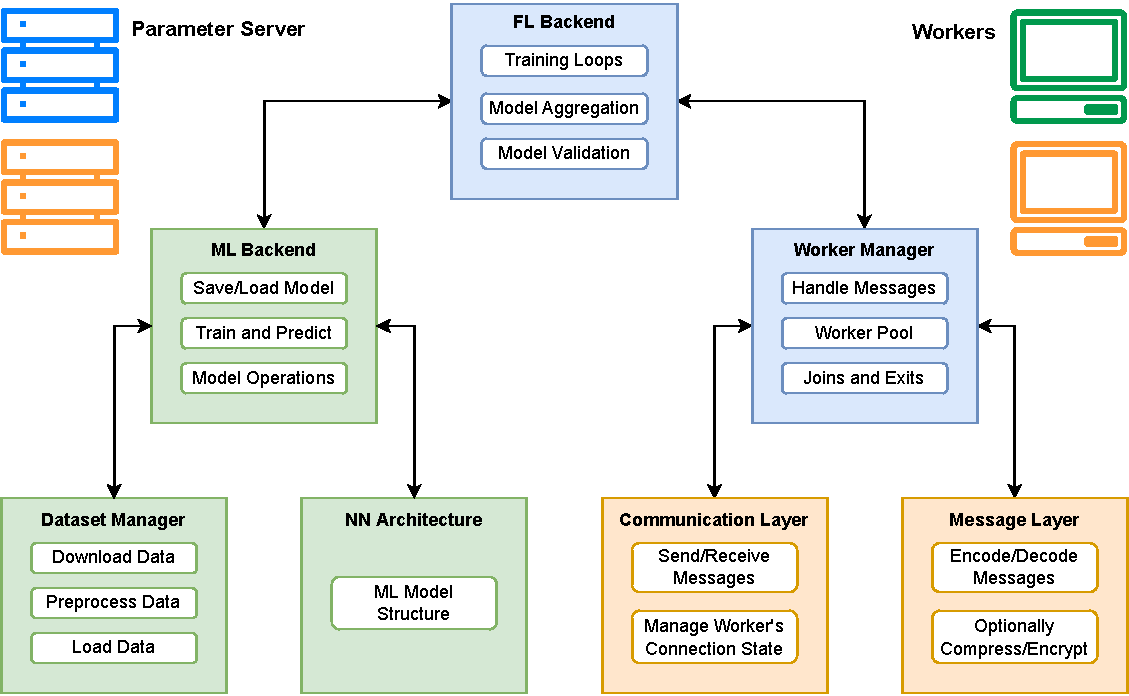
\includegraphics[width=\textwidth]{figs/modules.pdf}
    \caption[Proposed FL Framework Architecture]{Conceptual design of the resilient \ac{fl} system, showcasing its modular components and detailing the roles of the Parameter Server and Workers as key entities. The color-coding helps identify the primary functions of each module within the overall framework.}
    \label{fig:architecture}
\end{figure}

The architecture consists of the following core modules, each serving a specific purpose in the overall system:

\textbf{FL Backend:} This module serves as the central component for the Federated Learning process logic. On the Parameter Server, it manages the global training loop, orchestrates rounds, and determines worker scheduling, aggregates model updates from workers, updates the global model state, and validates it. On the worker side, it manages the local training loop and interaction with the server or peers, depending on the algorithm. It uses the \textit{ML Backend} for model interactions and the \textit{Worker Manager} to interact with workers.

\textbf{ML Backend:} This module provides an abstraction layer for the underlying \ac{ml} framework, making the rest of the framework independent of the specific library used. It handles the \ac{ml} model, offering interfaces for common operations such as saving/loading the model, training the model on local data, making predictions, and other general model operations like accessing weights or gradients. It employs the \textit{Dataset Manager} to retrieve data and the \textit{Neural Network Architecture} to define the model.

\textbf{Dataset Manager:} Responsible for all aspects related to handling data on the client devices. It oversees the data extraction process from local storage, potentially managing tasks like downloading (if data needs to be fetched), preprocessing the data, and loading split data batches for training, validation, and testing. It supplies processed data samples to the \textit{ML Backend}.

\textbf{Neural Network Architecture:} This module defines the structure of the \ac{ml} model being trained. It contains the specifications for the layers and connections of the \ac{nn} and is used by the \textit{ML Backend} to create the model instance before training starts. Separating this allows for straightforward swapping of model architectures for the same dataset or \ac{fl} scenario.

\textbf{Worker Manager:} Primarily located on the Parameter Server, this module manages the pool of participating client devices (workers). It tracks connected workers, handles joins/disconnects from the network, and manages the worker subpool used for each training round (particularly in client-selection scenarios), making it a key component in ensuring the system's elasticity and fault tolerance. It interacts with the workers using the \textit{Communication Layer} and the \textit{Message Layer}, allowing it to encode a message once and send it to multiple workers.

\textbf{Communication Layer:} This vital module handles all network communication between any nodes in the system, including the server and workers. It provides an abstract send and receive interface, concealing the complexities of the specific communication protocol employed. Importantly, this layer is also responsible for providing fundamental resilience to the system by managing connection status, addressing message delivery issues, and incorporating protocol-specific fault tolerance features.

\textbf{Message Layer:} Conceptually positioned below the Communication Layer, this module is responsible for defining the format and processing the content of exchanged messages. It includes functionalities to encode and decode messages and can optionally perform data compression and encryption of model updates or other exchanged information to enhance efficiency and security.

Having detailed the individual roles of the core modules, it is important to explicitly highlight how their collaborative design fulfills the system requirements outlined in Section \ref{sec:system_requirements_and_comparison}. Resilience is a key outcome, achieved through the Worker Manager's dynamic worker pool management and task rescheduling capabilities, ensuring training continuity despite node failures or disconnections. 

The Communication Layer (including the Message Layer for secure and efficient data transfer) further contributes by providing robust fault detection and handling mechanisms. 

Modularity is inherently built into the framework: the ML Backend abstracts diverse machine learning libraries, the FL Backend supports various federated learning algorithms, and the Communication Layer (with its various protocol implementations) allows for flexible integration of communication paradigms. This architectural flexibility, combined with the structured logging by modules like the Worker Manager and FL Backend, facilitates comprehensive Analysis of system performance and training progress. 

The framework's commitment to Code and Documentation is demonstrated by its open-source availability on GitHub and PyPI, alongside its intuitive \ac{cli} tools, making it accessible for researchers and practitioners to understand, use, and extend. Further technical details regarding the implementation of these design choices, including software stack and specific mechanisms, are provided in Chapter \ref{chap:implementation}. 

\section{Communication Strategies}

To further illustrate the proposed architecture's dynamic interactions and resilience mechanisms, particularly in worker participation and task management, we detail the communication sequences during key worker lifecycle events: initial join, network disconnection, and training round participation.

Coordinated by the core modules, these sequences demonstrate the framework's robustness in dynamic environments with fluctuating worker availability.

\subsection{Worker Join Sequence}

When a new worker connects to the system, it undergoes a registration process with the Parameter Server. This handshake establishes its identity and prepares it for participation in the training rounds. This sequence involves the worker initiating contact, the Parameter Server assigning it a unique identifier and a run identifier, and the worker confirming its registration by sending initial metadata before becoming available for tasks. 

The underlying communication protocol primarily handles the initial steps, while the subsequent metadata exchange and readiness signaling involve the Message Layer and Worker Manager. The detailed steps are illustrated in the sequence diagram in Figure~\ref{fig:seq:worker_joins}.

\begin{figure}[!htb]
    \centering
    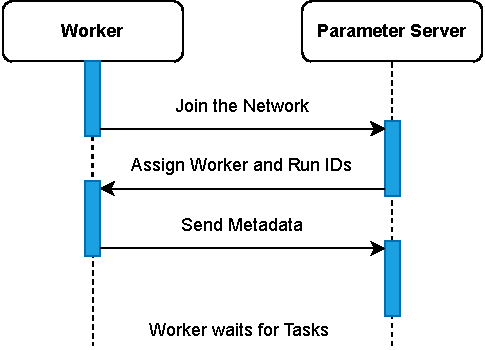
\includegraphics[width=0.5\textwidth]{figs/worker_joins.pdf}
    \caption[Worker Join Sequence in Federated Learning]{Communication sequence illustrating how a worker joins the \ac{fl} system by initiating contact, the Parameter Server assigning unique identifiers, the worker sending initial metadata, and finally, the worker becoming ready to receive tasks.}
    \label{fig:seq:worker_joins}
\end{figure}

\subsection{Worker Leaves Sequence}

Workers may leave the \ac{fl} system either gracefully (sending an explicit disconnect message) or abruptly (due to unexpected disconnections or failures). The framework's resilience relies on the Parameter Server's ability to detect both scenarios and update the active worker pool managed by the Worker Manager accordingly. If a worker sends a leave message, the server receives and processes it. If a worker disconnects unexpectedly, the protocol-specific mechanisms in the Communication Layer detect the loss of connection. Figure~\ref{fig:seq:worker_leaves} illustrates the communication flow for a worker leaving the system.

\begin{figure}[!htb]
    \centering
    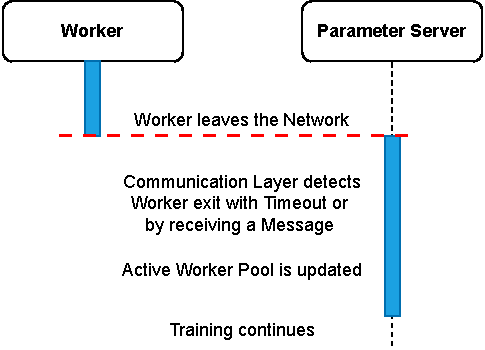
\includegraphics[width=0.5\textwidth]{figs/worker_leaves.pdf}
    \caption[Worker Leaves Sequence in Federated Learning]{Communication sequence illustrating how a worker leaves the \ac{fl} system. The Parameter Server's communication layer detects the worker's exit, either through an explicit message or a timeout, which triggers an update to the active worker pool and allows the training process to continue uninterrupted.}
    \label{fig:seq:worker_leaves}
\end{figure}


\subsection{Work Cycle Sequence}

This sequence depicts the typical communication flow when a worker receives and processes a task during a training round. It starts with the Parameter Server sending the necessary data or model parameters for the task. The worker then performs its local computation (training on its data). Upon completion, the worker returns its results or model updates to the Parameter Server and waits for future messages. The sequence diagram in Figure~\ref{fig:seq:worker_works} illustrates this successful cycle.

\begin{figure}[!htb]
    \centering
    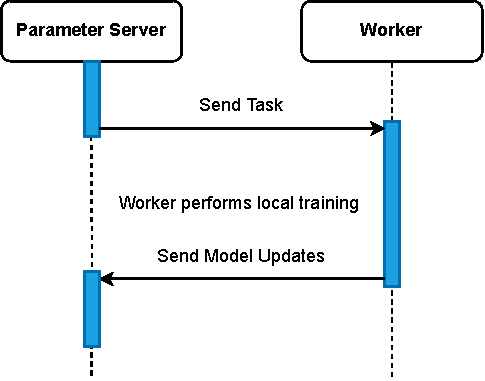
\includegraphics[width=0.5\textwidth]{figs/worker_works.pdf}
    \caption[Worker Task Completion Sequence]{Communication sequence illustrating a worker successfully receiving and completing a task within the \ac{fl} system. The process shows the Parameter Server sending a task, the worker performing local training, and then sending model updates back to the server.}
    \label{fig:seq:worker_works}
\end{figure}

A critical aspect of resilience is handling failures during the work cycle. The Parameter Server must detect if a worker fails after receiving a task but before successfully submitting its results. Depending on the \ac{fl} algorithm (synchronous vs. asynchronous) and the resilience mechanisms implemented (e.g., completion thresholds, task rescheduling by the Worker Manager), the framework adapts to continue training. The sequence diagram in Figure~\ref{fig:seq:worker_fails_work} shows an example of this failure scenario and server detection.

\begin{figure}[!htb]
    \centering
    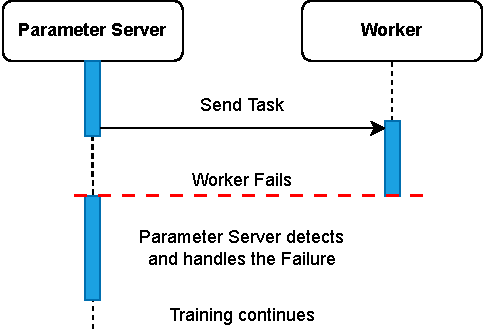
\includegraphics[width=0.5\textwidth]{figs/worker_fails_work.pdf}
    \caption[Worker Failure and Server Detection]{Communication sequence illustrating a worker failure during task execution and the Parameter Server's subsequent detection and handling of this event. This ensures that the \ac{fl} training process can continue despite the disruption.}
    \label{fig:seq:worker_fails_work}
\end{figure}



\section{SWOT Analysis}
\label{sec:swot_analysis}

To provide a comprehensive understanding of the proposed architecture, a SWOT analysis was conducted to evaluate its internal strengths and weaknesses alongside external opportunities and threats. The SWOT analysis is summarized in Table~\ref{tab:swot} and it serves as a guide for future development and evaluation, highlighting areas for improvement and potential risks that must be addressed.

\begin{table}[!htb]
    \caption[SWOT Analysis of the Proposed Solution]{A comprehensive SWOT analysis of the proposed \ac{fl} framework, detailing its internal strengths and weaknesses, alongside external opportunities and threats. This provides a balanced view of its potential and limitations for future development.}
    \label{tab:swot}
    \centering
    \begin{tabular}{Sc | Sc Sc}
    & \textbf{Helpful} & \textbf{Harmful} \\
    \toprule
    \textbf{Internal} & 
    \begin{tabular}[c]{@{}c@{}}\textbf{Strengths} \\
        \addlinespace
        \begin{tabular}[c]{@{}c@{}}Resilient, highly modular \\ and easy to use\end{tabular} \\
    \end{tabular} &
    \begin{tabular}[c]{@{}c@{}}\textbf{Weaknesses} \\ 
        \addlinespace
        \begin{tabular}[c]{@{}c@{}}Validation is limited to \\ the simulation environment\end{tabular} \\
    \end{tabular} \\
    \midrule
    \textbf{External} &
    \begin{tabular}[c]{@{}c@{}}\textbf{Opportunities} \\ 
        \addlinespace
        \begin{tabular}[c]{@{}c@{}}Easy to extend and \\ integrate with other systems\end{tabular} \\
    \end{tabular} &
    \begin{tabular}[c]{@{}c@{}}\textbf{Threats} \\ 
        \addlinespace
        \begin{tabular}[c]{@{}c@{}}Scalability may \\ be limited \end{tabular} \\
    \end{tabular} \\
    \bottomrule
\end{tabular}
\end{table} 


The main strengths are: resilience, modularity, and ease of use. The system is designed to handle dynamic network conditions, ensuring seamless operation even when nodes join or leave the network. The architecture features a highly modular design, working as a puzzle where each piece can be replaced or extended without affecting the other modules. 

Despite its strengths, the system has certain internal weaknesses that may affect its practical utility. The proposed solution will be evaluated in a simulated environment using \acp{vm}. While this provides valuable initial insights, it does not fully replicate real-world conditions. Challenges such as hardware diversity, network instability, and scalability in large-scale deployments are not fully captured in the simulation, limiting the system's validation.

The external opportunities for the proposed solution are vast, as the system is designed to be easily extended and integrated with other systems. This flexibility allows for the integration of new \ac{fl} algorithms, communication protocols, and \ac{ml} models, providing a versatile platform for research and development. The system's modularity also enables the integration of new features and functionalities, allowing for continuous improvement and adaptation to changing requirements.

Finally, the system faces certain external threats that may impact its long-term viability. Despite the system being designed to be scalable, environments with a larger number of workers than the simulation environment may pose challenges. The system's performance may degrade as the number of workers increases, affecting the overall efficiency and effectiveness of the \ac{fl} process. 

